\section{Requisitos funcionais - Diagramas UML}

\subsection{Diagrama de casos de uso}
\begin{figure}[!h]
\centering
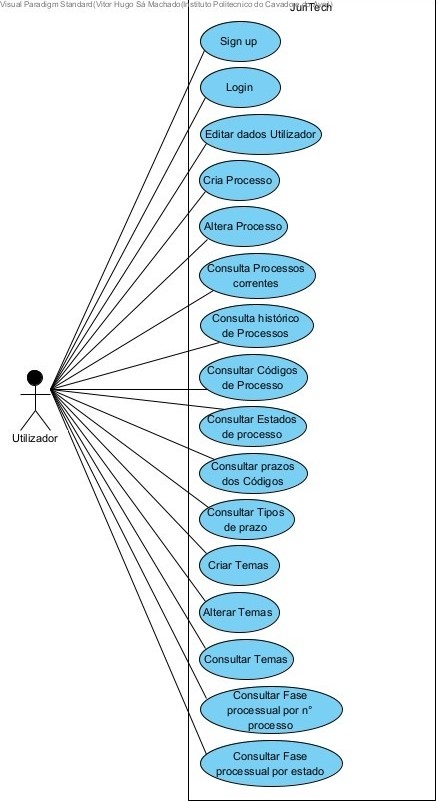
\includegraphics[width=0.5\textwidth]{Figuras/caso_de_uso_1.jpg}
\caption{Diagrama de caso de usos(1)}
\label{d.cdu}
\end{figure}
\newpage

\begin{figure}[!h]
\centering
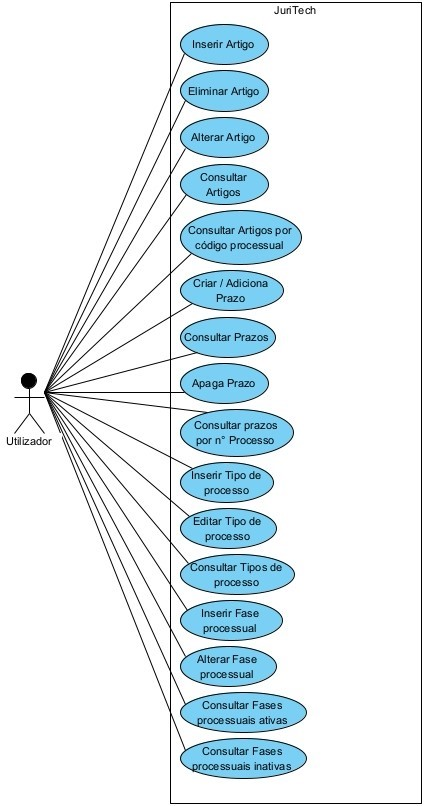
\includegraphics[width=0.5\textwidth]{Figuras/caso_de_uso_2.jpg}
\caption{Diagrama de caso de usos(2)}
\label{d.cdu}
\end{figure}
\newpage

\subsection{Diagrama de componentes}
\begin{figure}[!h]
\centering
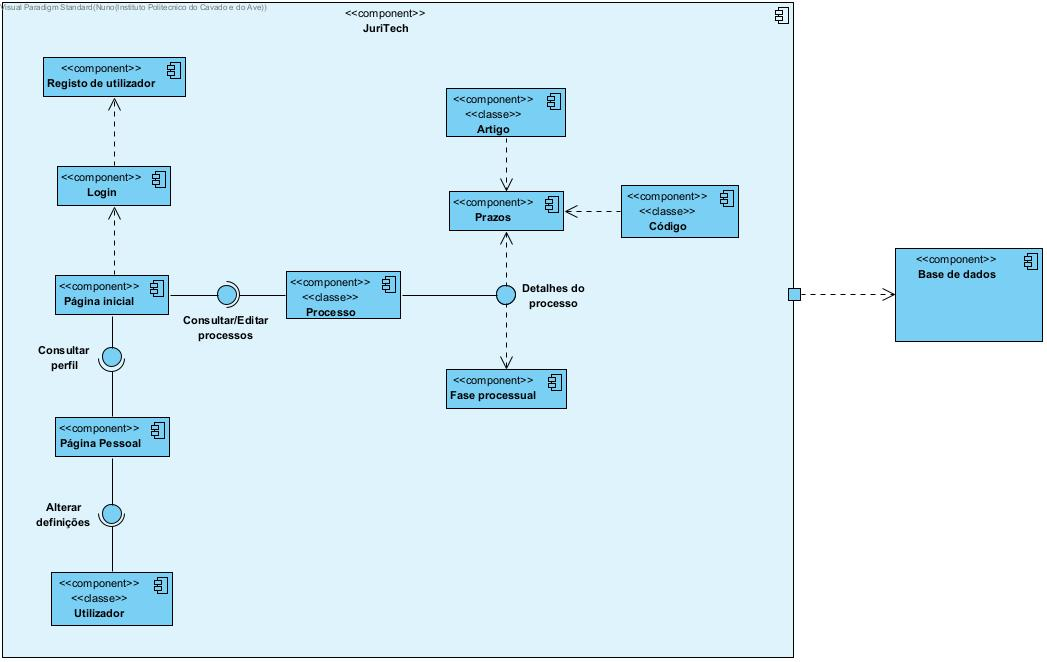
\includegraphics[width=0.9\textwidth]{Figuras/d.componentes.jpg}
\caption{Diagrama de componentes}
\label{d.componentes}
\end{figure}
\newpage

\subsection{Diagrama de Visão geral de interação}
\begin{figure}[!h]
\centering
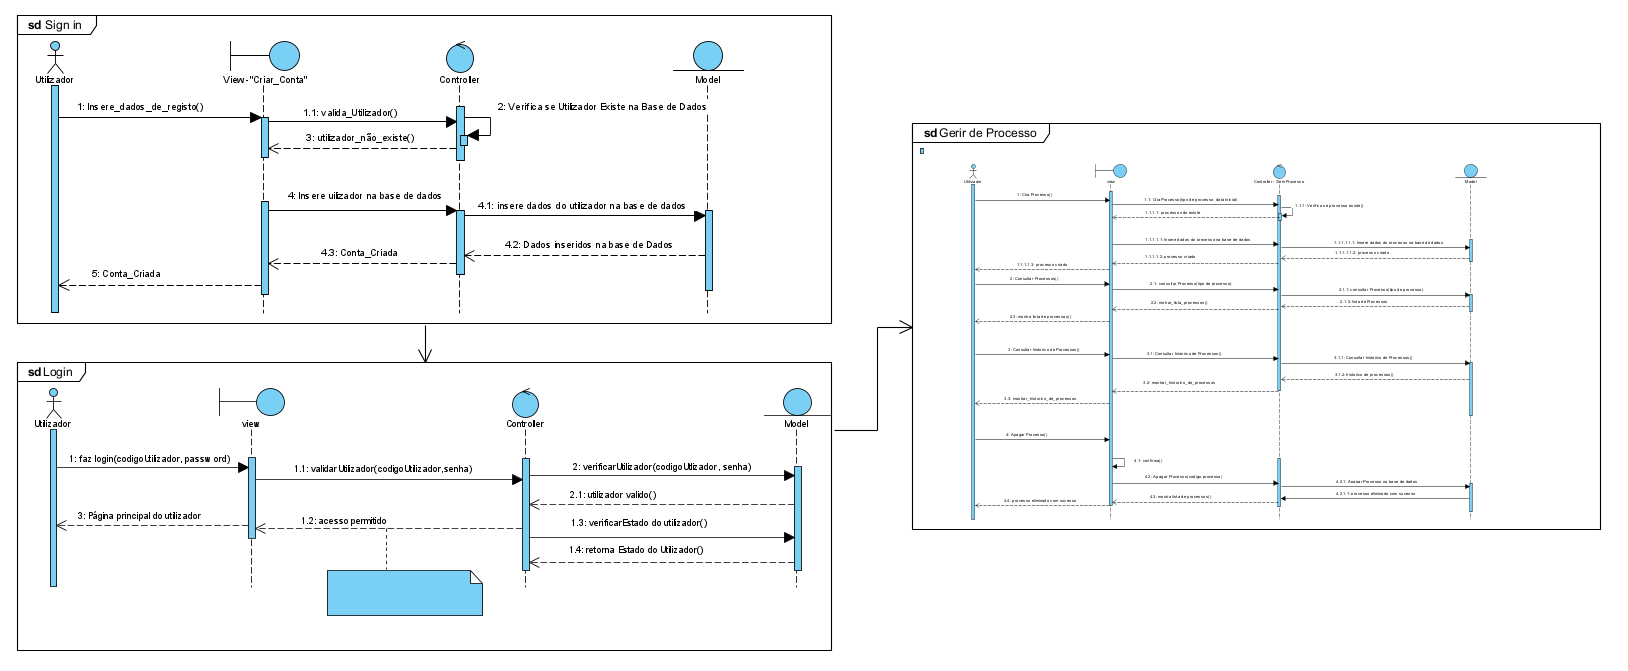
\includegraphics[width=1.1\textwidth]{Figuras/d. visão geral de interação.png}
\caption{Diagrama de visão geral de interação}
\label{d.componentes}
\end{figure}

\begin{figure}[!h]
\centering
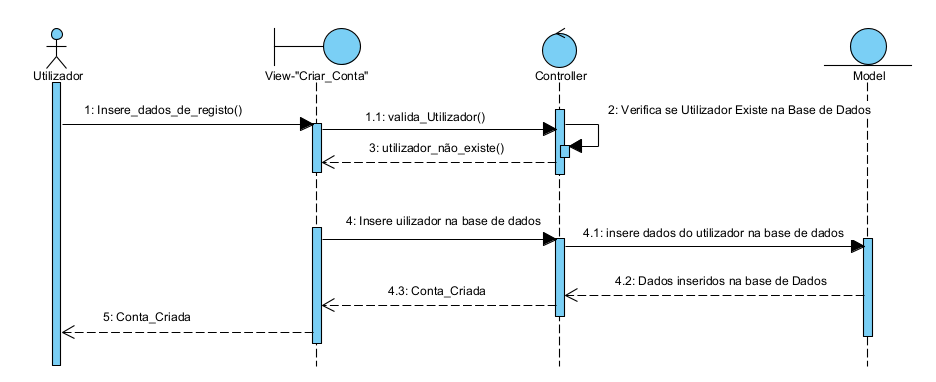
\includegraphics[width=1.1\textwidth]{Figuras/d. visão geral de interação_sign up.png}
\caption{Diagrama de visão geral de interação "Sign Up"}
\label{d.componentes}
\end{figure}

\begin{figure}[!h]
\centering
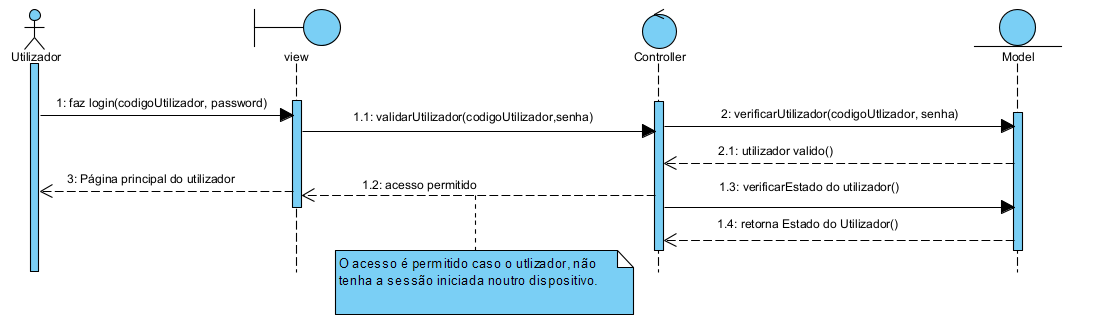
\includegraphics[width=1.1\textwidth]{Figuras/d. visão geral de interação_login.png}
\caption{Diagrama de visão geral de interação "Login"}
\label{d.componentes}
\end{figure}

\begin{figure}[!h]
\centering
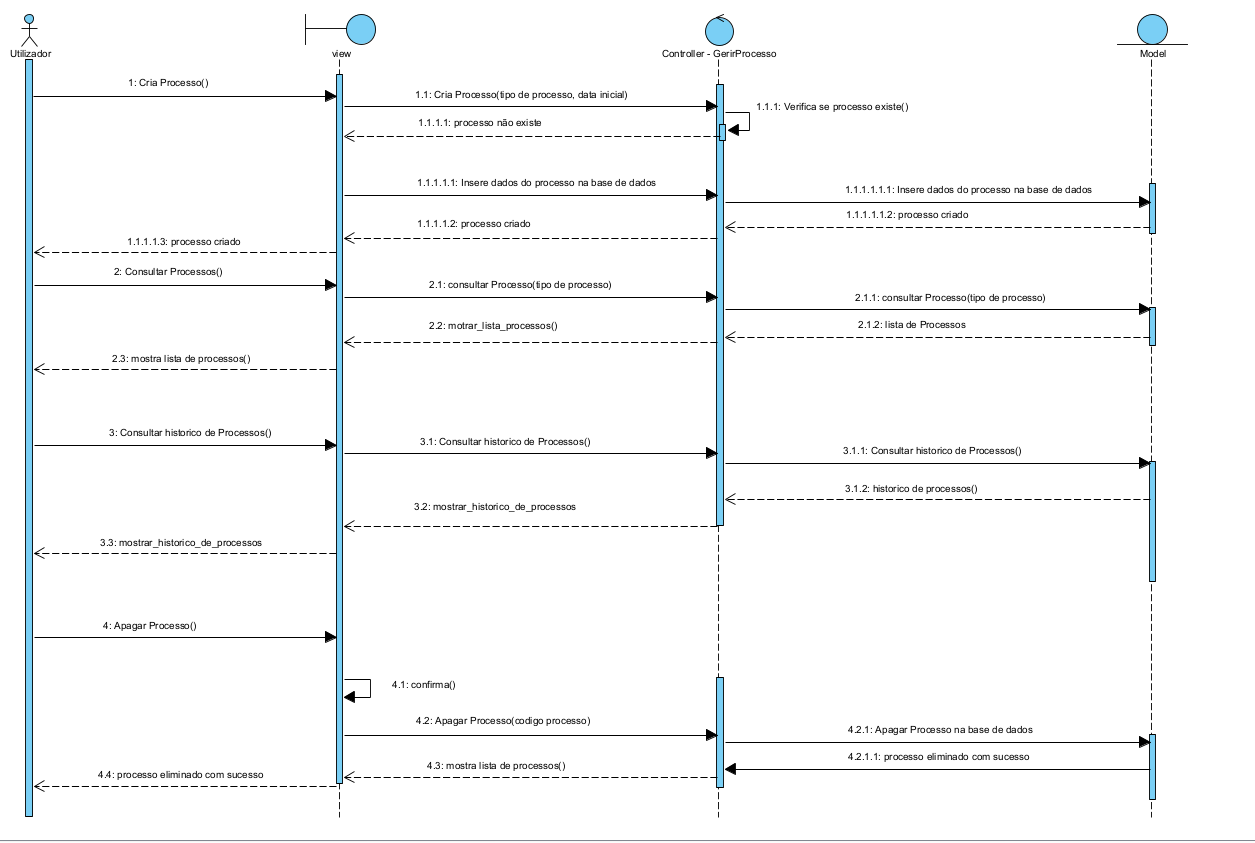
\includegraphics[width=1.1\textwidth]{Figuras/d. visão geral de interação_Gerir Processos.png}
\caption{Diagrama de visão geral de interação "Gerir Processo"}
\label{d.componentes}
\end{figure}

\clearpage
\subsection{Diagrama de Classes UML}
\begin{figure}[!h]
\centering
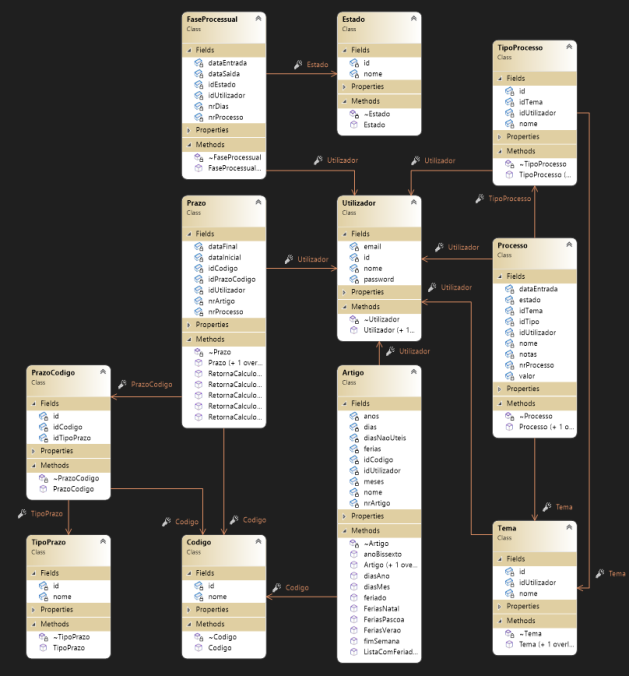
\includegraphics[width=17cm]{Figuras/Class Diagram.png}
\caption{Diagrama de classes UML}
\label{d.componentes}
\end{figure}
\newpage

\subsection{Diagrama de Entidade relação}
\begin{figure}[!h]
\centering
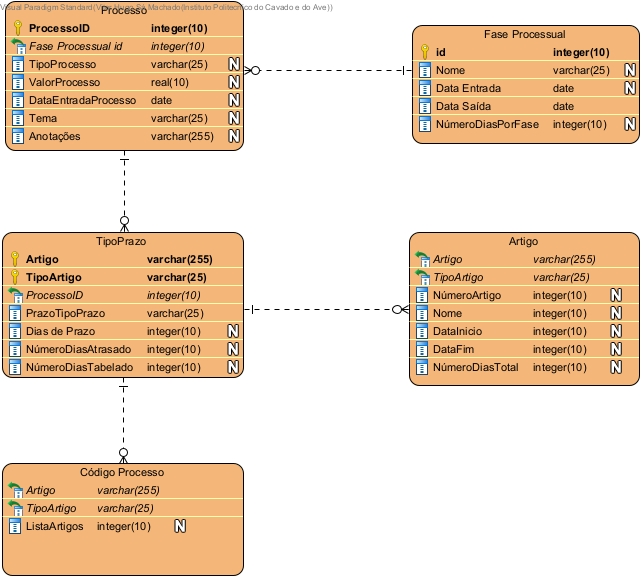
\includegraphics[width=17cm]{Figuras/diagrama entidade relação.jpg}
\caption{Diagrama entidade relação - diagrama da futura base dados}
\label{d.componentes}
\end{figure}






